\section{Scénář používání}

% Vložení SVG souboru tady v tomhle Overleaf projektu prostě nefunguje
\begin{figure}
    \begin{centering}
        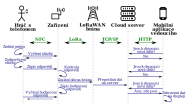
\includegraphics[width=1\textwidth]{Figures/communication-diagram}
        \caption{Komunikační diagram}
        \label{fig:Usage_comm_diag}
    \end{centering}
\end{figure}

Diagram \ref{fig:Usage_comm_diag} popisuje jak je zařízení prakticky používáno.

Zařízení je nejprve vedoucími umístěno v terénu. Poté k němu přicházejí hráči, vybaveni  telefony s nainstalovanou mobilní aplikací. Hráč přijde k zařízení, spustí na svém telefonu aplikaci, zadá své jméno a přiloží ji k NFC rozhraní zařízení. Aplikace z NFC tagu (resp. z jeho paměti) vyčte soutěžní otázku a zobrazí ji hráči. Hráč zadá odpověď, a podruhé přiloží telefon k zařízení -- tentokrát aplikace zapíše hráčovu odpověď a jeho jméno do NFC tagu.
Zařízení v tuto dobu NFC tag monitoruje, a ve chvíli kdy aplikace dokončí zápis zapsaná data vyčte. Poté posoudí správnost odpovědi, a výsledek zapíše do NFC tagu. Zároveň odešle do LoRaWAN sítě zprávu s hráčovým jménem, jeho odpovědí a časem kdy odpověď zadal.
Hráč po zápisu odpovědi do NFC tagu k němu přiloží svůj telefon potřetí, a aplikace vyčte vyhodnocení jeho odpovědi.

LoRaWAN síť se mezitím postará o to aby byla zpráva vyslaná zařízením dopravena na server a zpřístupněna skrze HTTP API. Tohoto API se mobilní aplikace vedoucího v pravidelných časových intervalech doptává na nová data, a jsou-li nějaká k dispozici, zobrazí je v seznamu na displeji.

\section{Části zařízení a jejich komunikace}

\begin{center}
     \textbf{<<zde bude doplněn diagram>>}
\end{center}

Jádrem celého zařízení je MCU, jež dle programu nahraném v jeho paměti komunikuje s ostatními částmi a zajišťuje celkovou funkci.

S LoRa modulem komunikuje skrze SPI sběrnici, ve které figuruje jako podřízené (Slave) zařízení, mikrokontrolér je v roli zařízení nadřízeného (Master). Pouze nadřízené zařízení může iniciovat komunikaci. Skrze standardní signály sběrnice (MISO, MOSI, SCK, CS) posílá mikrokontrolér LoRa modulu příkazy, konfiguruje jej a vyčítá odpovědi. Protože SPI sběrnice nenabící podřízeným zařízením možnost asynchronně informovat zařízení nadřízené, jsou použity dva další signály -- BUSY, kterým modul dává najevo že není připraven přijímat další data, a DIO1 (taktéž označován jako IRQ), kterým mikrokontroléru oznamuje že má k dispozici data přijatá přes rádiovou komunikaci.

Druhou použitou sběrnicí je I\textsuperscript{2}C. Ta používá dva signálové vodiče, SDA a SCL, ke kterým může být připojeno až 127 zařízení. Zde je na na sběrnici jedno nadřízené (Master) zařízení, tím je mikrokontrolér, a více, konkrétně dvě, podřízená (Slave) zařízení, těmi jsou NFC tag a LCD displej. Tato situace je na I\textsuperscript{2}C sběrnici nejčastější, nikoli ale jediná možná -- I\textsuperscript{2}C podporuje i více nadřízených zařízení na jedné sběrnici. Podobně jako u SPI, pouze nadřízené zařízení může iniciovat komunikaci, podřízená pouze čekají až budou ke komunikaci vyzvána.

LCD displej je z hlediska komunikace jednoduché zařízení -- mikrokontrolér pouze zapisuje do jeho paměti, a to co do ní zapíše se na displeji zobrazí. Použitý displej je textový, se čtyřmi řádky po dvaceti znacích a možností definovat několik vlastních znaků (toho však není využito).

Druhý přes I\textsuperscript{2}C připojený modul je dynamický NFC tag. Ten, podobně jako LoRa modul, umí notifikovat mikrokontrolér o asynchronních událostech skrze zvláštní signál, GPO. NFC modul nabízí možnost výběru jedné z několika předdefinovaných událostí, o které skrze GPO signál mikrokontrolér informuje. Této funkce zařízení využívá.

Poslední použitou sběrnicí, také sériovou, je UART. Ta je použita pro (jednosměrné) zasílání dat do PC, to slouží především pro přehled o činnosti zařízení při úpravách programu. Je možno ji použít i v terénu, a to použitím UART-Bluetooth modulu, například HC-05. V takovém případě je pro zobrazení dat nejčastěji využíván mobilní telefon s přísloušnou aplikací.
